\chapter{Laboratorium II}\label{ch:lab2}

\section{Wybrany sprzęt}\label{sec:lab2-hw}

System modułów \emph{Grove} jest~wykorzystany w~dwóch laboratoriach, w~związku z~czym jego~opis znajduje~się w~sekcji
przodującej (\ref{subsec:grove}).
W~niniejszym laboratorium zostały użyte dwa~urządzenia współpracujące z~modułem \emph{Grove Base HAT}.

Głównym elementem zestawu laboratoryjnego jest~czujnik wykorzystujący czas propagacji fal ultradźwiękowych do~pomiaru
odległości.
Sensor emituje krótki sygnał ultradźwiękowy, a~następnie nasłuchuje momentu powrotu echa fali od~przeszkody, co~pozwala
na~obliczenie dystansu przebytego przez~falę, a~zarazem odległości od~przeszkody.

Do~wyświetlenia wyników pomiaru wybrany został wyświetlacz LCD $2\,\times\,16$ komórek o~wielkości komórki
$8\,\times\,5$ pikseli.
Długość \num{16} komórek pozwala na~wyświetlenie mierzonej wartości wraz z~jednostką i~krótkim opisem, a~druga linia
może~służyć do~danych pomocniczych lub~drugiego rekordu.
Wyświetlacz~ten jest~zaprojektowany do~obsługi tekstu i~nie~można wykorzystać pikseli do~dowolnego rysowania.

\section{Dodatkowe oprogramowanie}\label{sec:lab2-sw}

\emph{Seeed-grove.py} to oficjalna biblioteka programistyczna zestawu \emph{Grove} w języku \emph{Python}.
Niestety nie jest ona dostępna przy~wykorzystaniu standardowego repozytorium bibliotek języka.
Kod biblioteki można zobaczyć jednak na~platformie \emph{GitHub}\thinspace\cite{grovelib}, dzięki~czemu nadal
możliwa~jest stosunkowo prosta instalacja (rys.~\ref{fig:seeed}) przy~użyciu stosunkowo nowych wersji oficjalnego
menedżera bibliotek.

\begin{figure}[H]
  \lstinputlisting[language=bash,label={lst:seeed}]{media/seeed.sh}
  \caption{Instalacja biblioteki \emph{grove} z~platformy \emph{GitHub}}
  \label{fig:seeed}
\end{figure}

\section{Rozwiązanie}\label{sec:lab2-sol}

Rysunek~\ref{fig:distancelab} to~fragment instrukcji przestawiający dwa z~zadań składających~się na~końcowy program
mierzący odległość do~obiektu przy~wykorzystaniu sensora ultradźwiękowego.
Pierwsze zadanie polega na~uzupełnieniu ciała funkcji wykorzystując podaną zmienną i~podstawowe prawa fizyki w~celu
otrzymania wartości odległości zmierzonej przez~czujnik ultradźwiękowy.
Drugie wyświetla obliczone wartości na~wyświetlaczu LCD -- z~powodu szybkiego odświeżania wykorzystując wyrównanie
danych bez~czyszczenia ekranu funkcją \emph{clear}.

\begin{figure}[H]
  \centering
  \includegraphics[width=0.9\linewidth]{media/distance_lab}
  \caption{Fragment instrukcji ``Odległość''}
  \label{fig:distancelab}
\end{figure}

Rysunek~\ref{fig:distance} przedstawia rozwiązanie zadania.
W~tym przypadku podana odległość jest~do~telefonu, którym~utworzone zostało zdjęcie, a~wyświetlacz jest~w~trakcie
zmiany wyświetlanej wartości.

\begin{figure}[H]
  \centering
  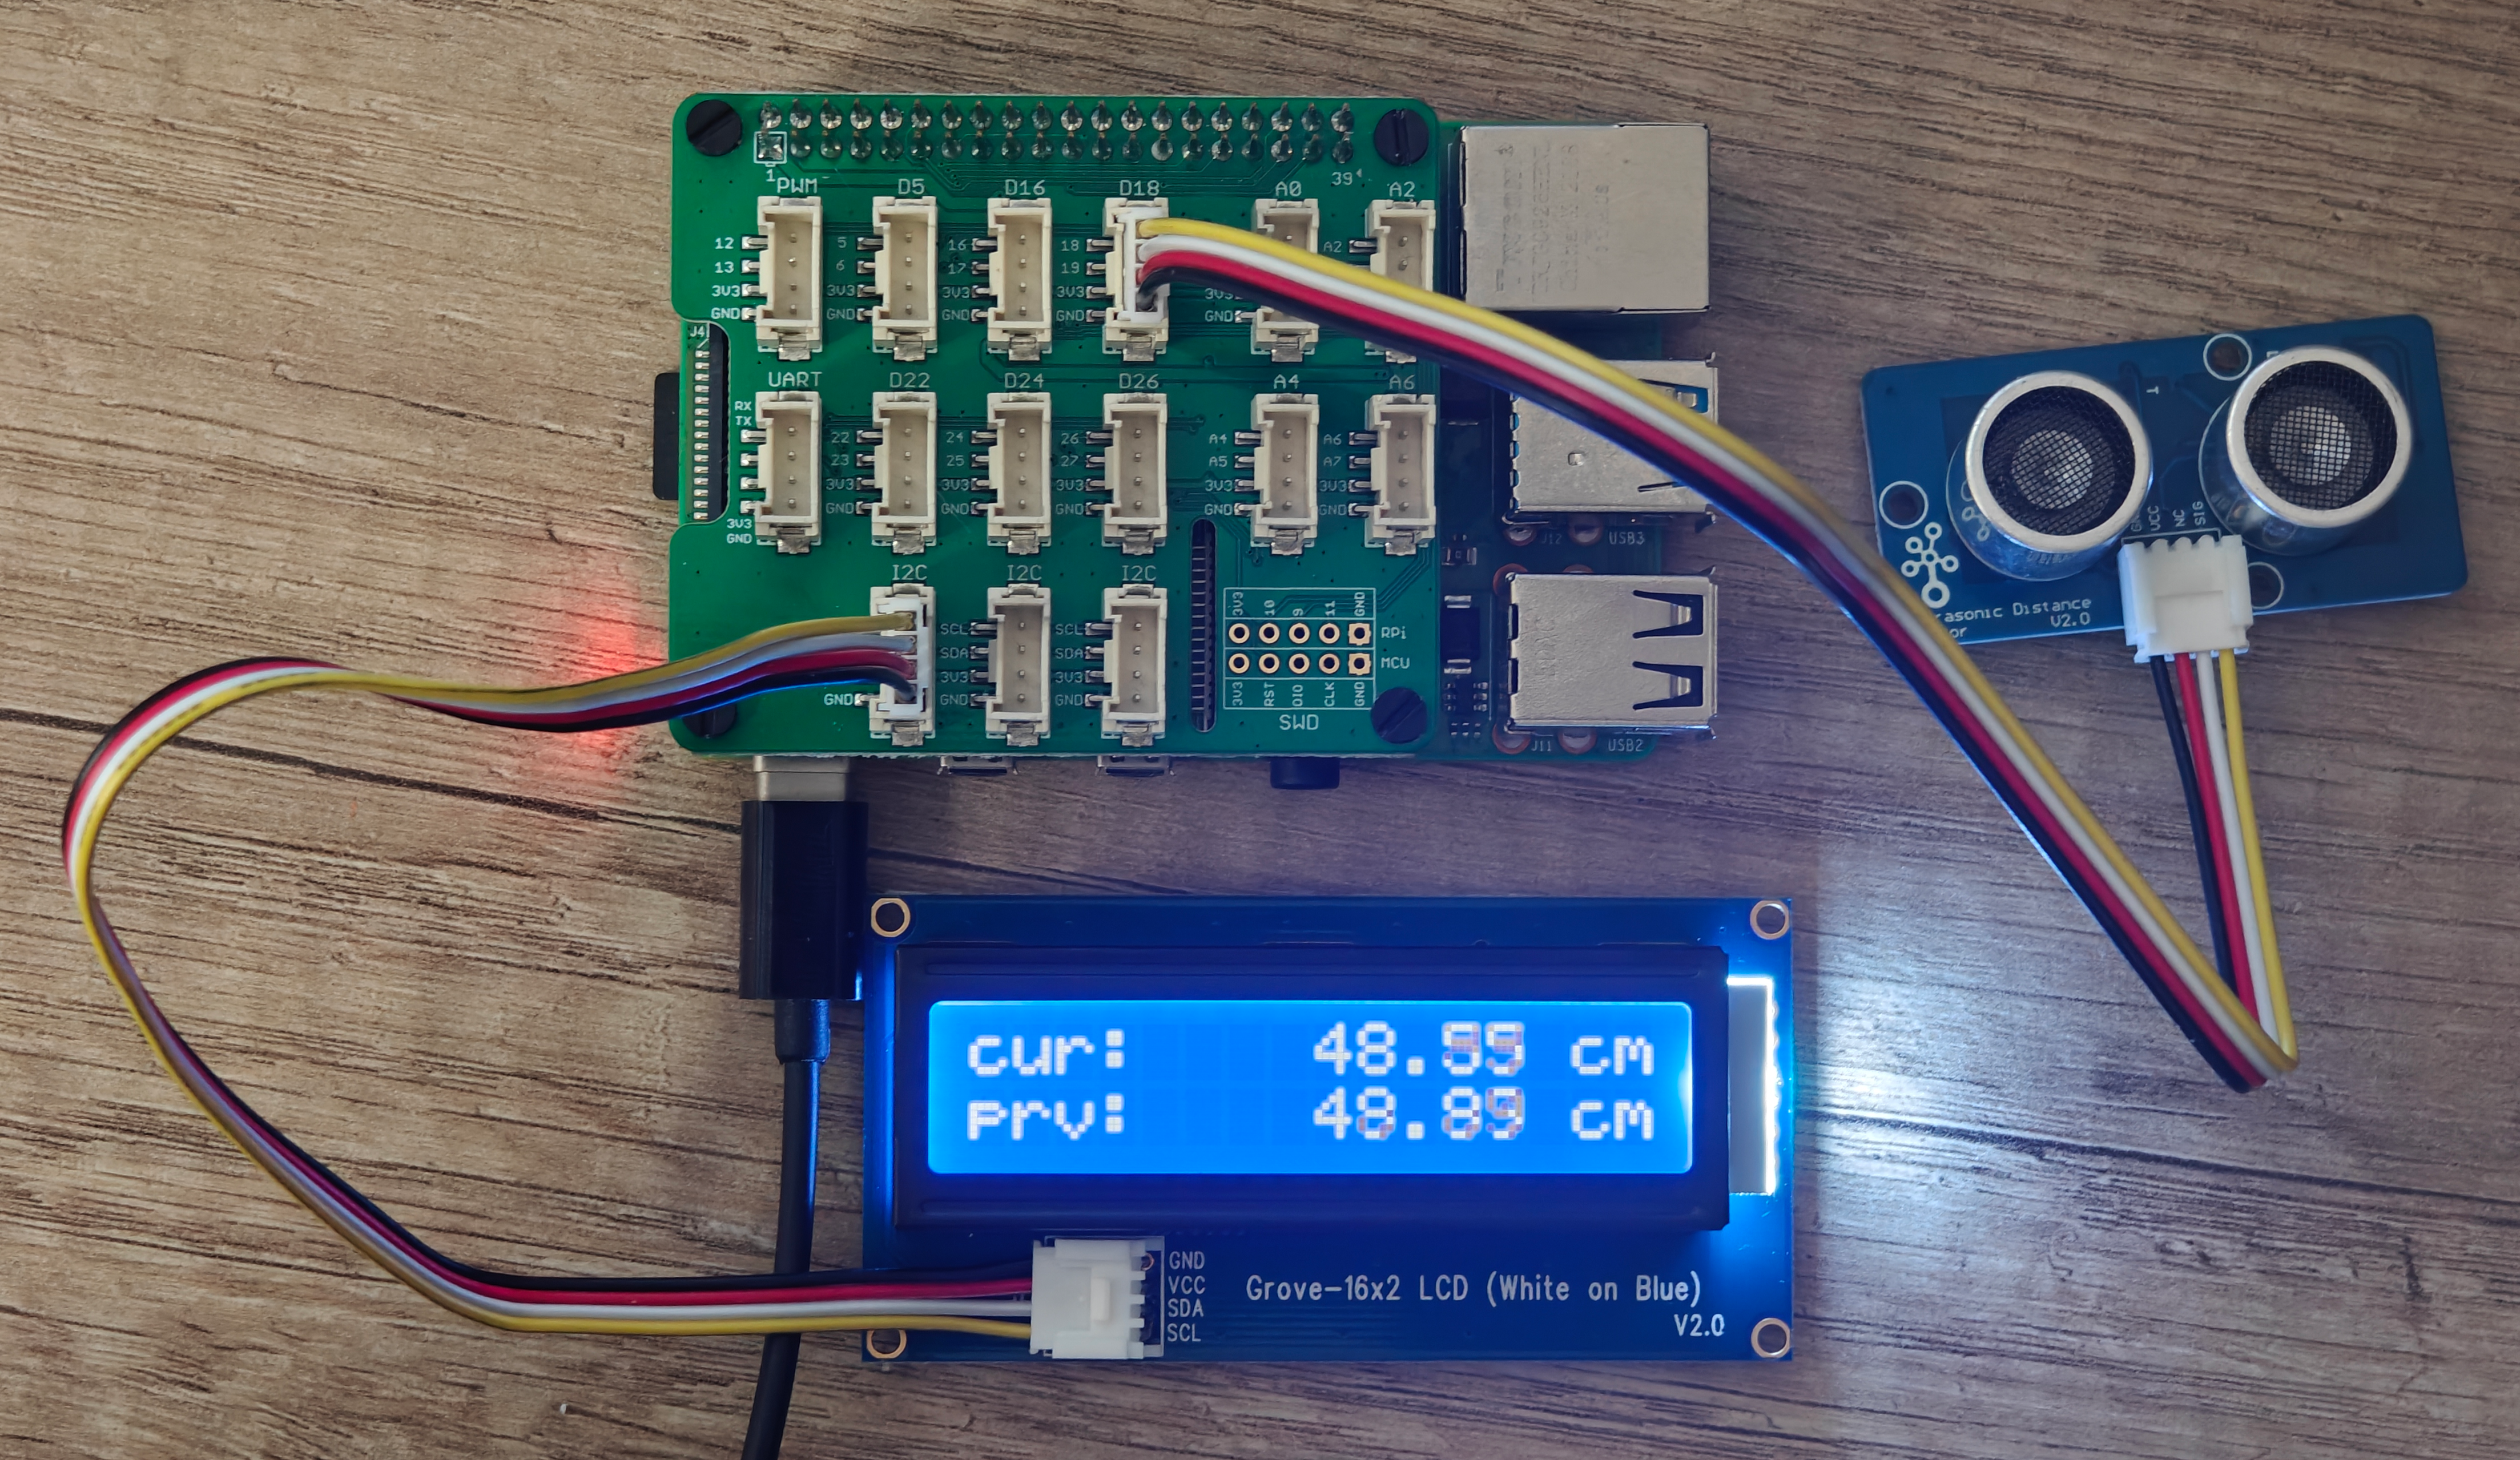
\includegraphics[width=0.6\linewidth]{media/distance}
  \caption{Uruchomiony program drugiego laboratorium}
  \label{fig:distance}
\end{figure}
